\section{Statement of Problem}
Task 2 utilizes a wave ray tracing algorithm and local bathymetry information, provided for Narragansett Bay, in order to propagate storm waves determined from task 1. In order to complete this task, simulations are conducted for the 20 and 50 year storms along with creating rays that intersect along the shoreline of Narragansett Beach. For the 20 year storm simulations, use the ray spacing on the beach to calculate a refraction coefficient for each section of beach. Then, using bathymetry data from a chart near the beach, estimate the beach slope. This is used along with the deep water wave properties and refraction coefficient to estimate the shoaling coefficient, breaking depth, and breaker height. 
\section{Hypotheses and Theories}

The direction a wave travels in can be influenced by the sea floor in shallow water. Refraction occurs when one part of a waves moves more quickly than another part. As waves increase 

\section{Solution of the Problem}

Using the supplied C functions and waveray.m, wave rays were propagated into Narragansett Beach under the conditions determined in Task 1. Twenty and fifty year predicted wave parameters were used to simulate the path lines extreme waves followed. Seen in CITE WAVEDIR FIGURE HERE, three predominant angles of incidence were determined from the supplied data. Waveray.m  was non-intuitive, and didn't allow for significant manipulation of the rendered area without ruining the data. A consequence of this was that our breaking wave characteristics were evaluated manually, and were not based off the simulation data.

Seen below, the simulated wave rays from all three angles of incidence experienced de-focusing as they approached the beach. Significant focusing can be observed in \ref{fig20y210deg} further south on the shoreline. 

\begin{figure}[H]
\centering
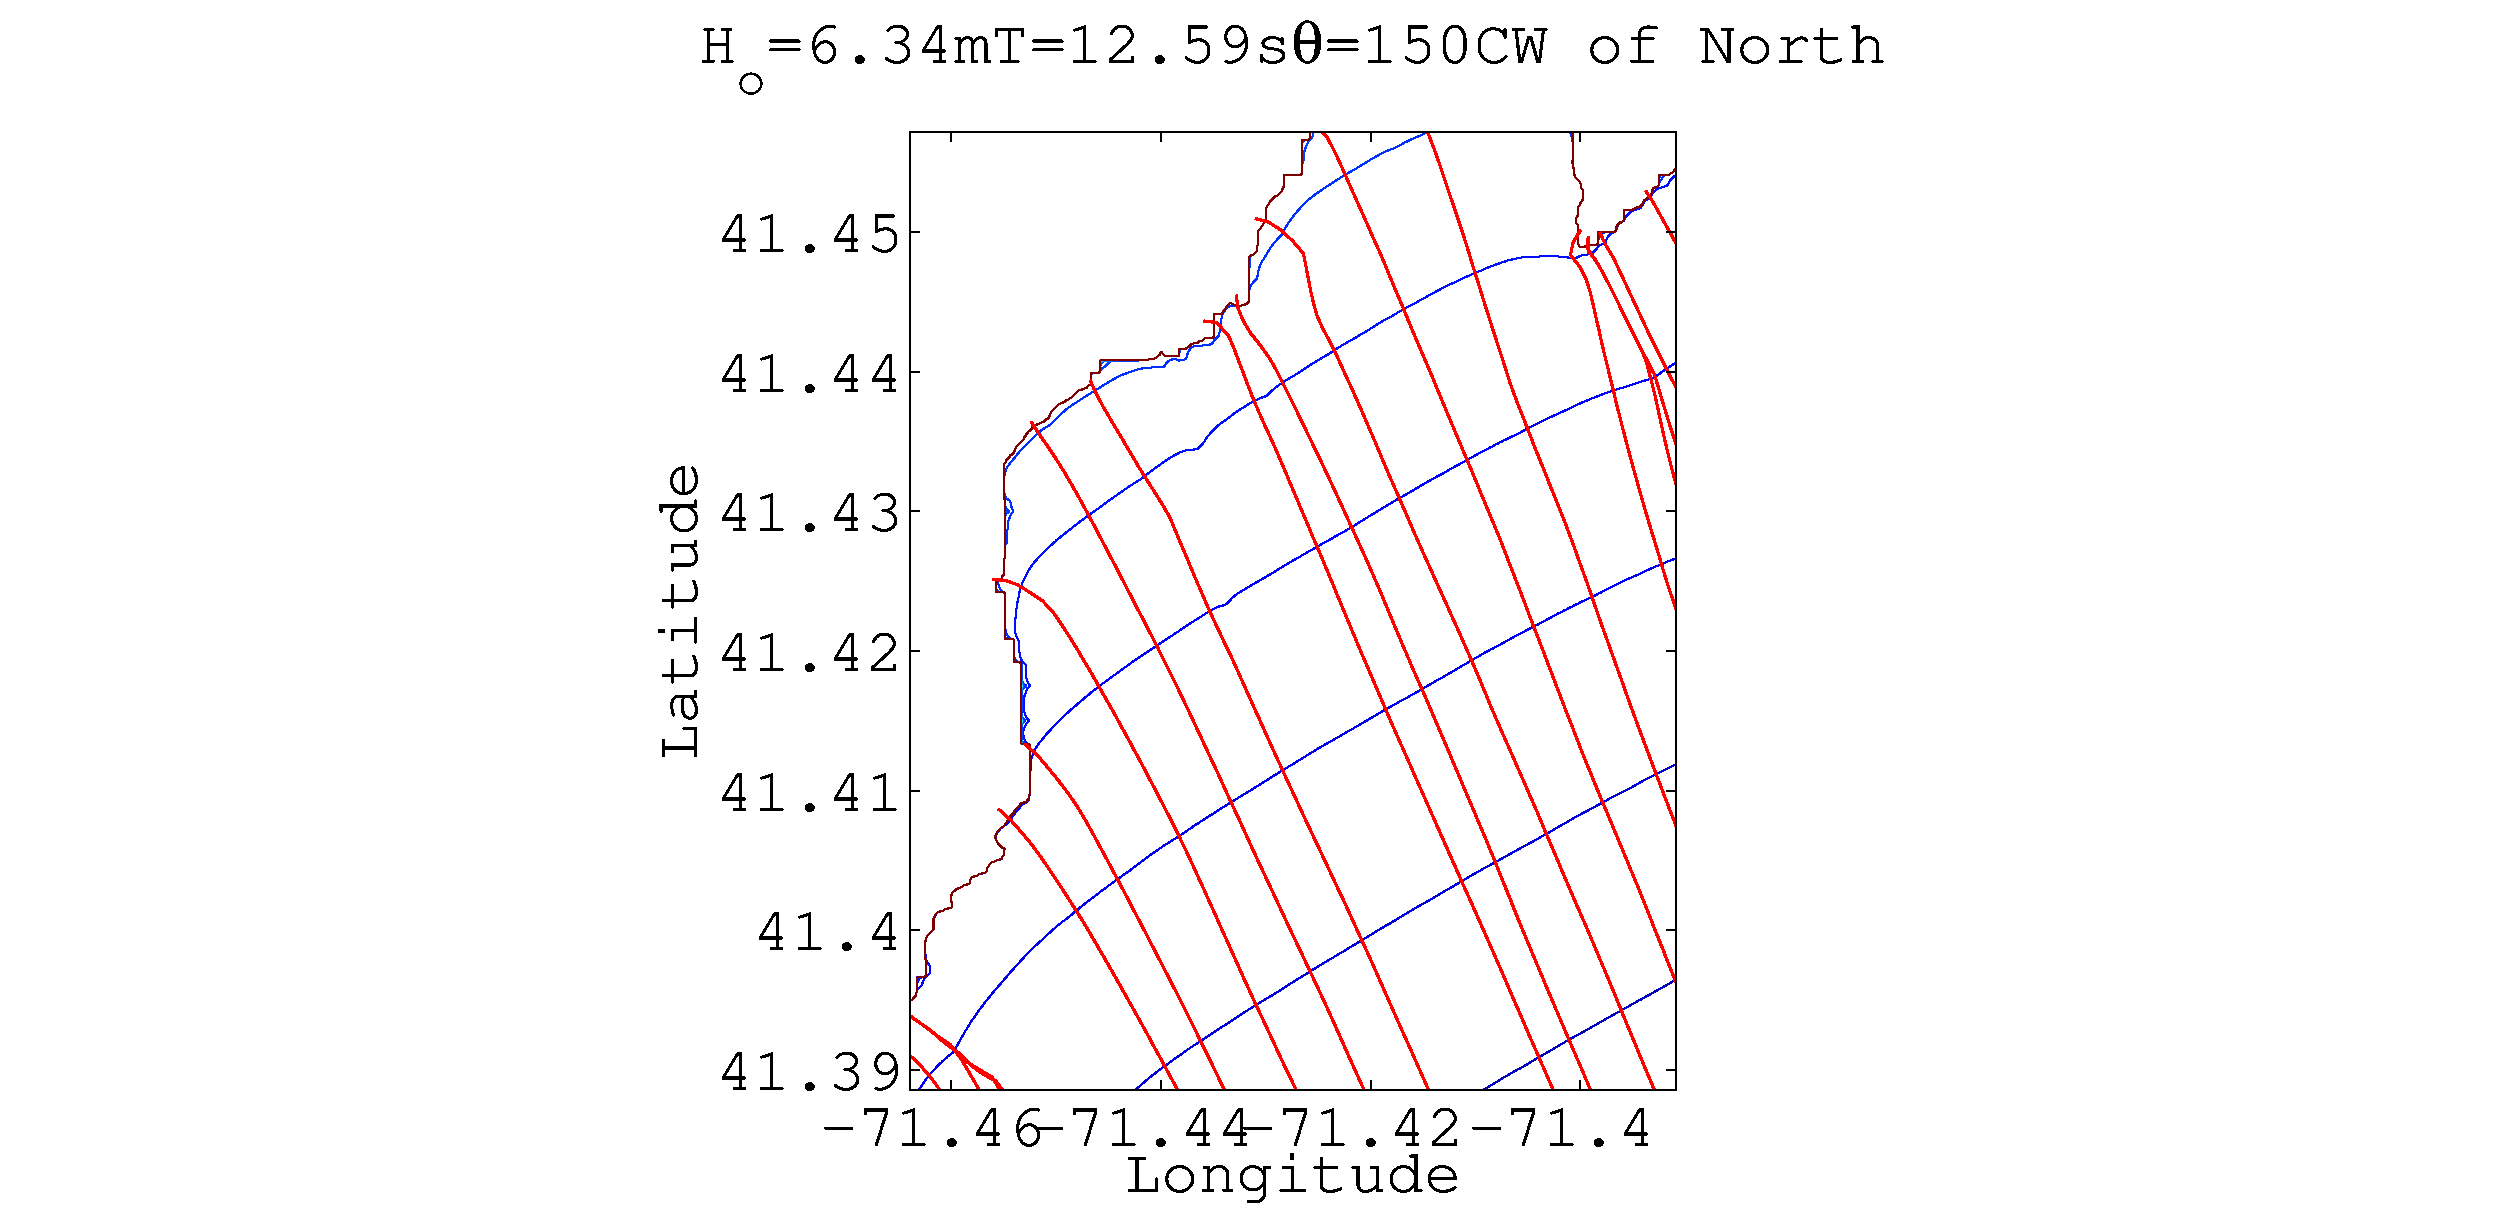
\includegraphics[width=1.0\textwidth]{./img/20y_150deg.eps}
\caption{Wave Ray 20y Expected Wave Parameters at 150 deg}
\label{fig:20y150deg}
\end{figure}

\begin{figure}[H]
\centering
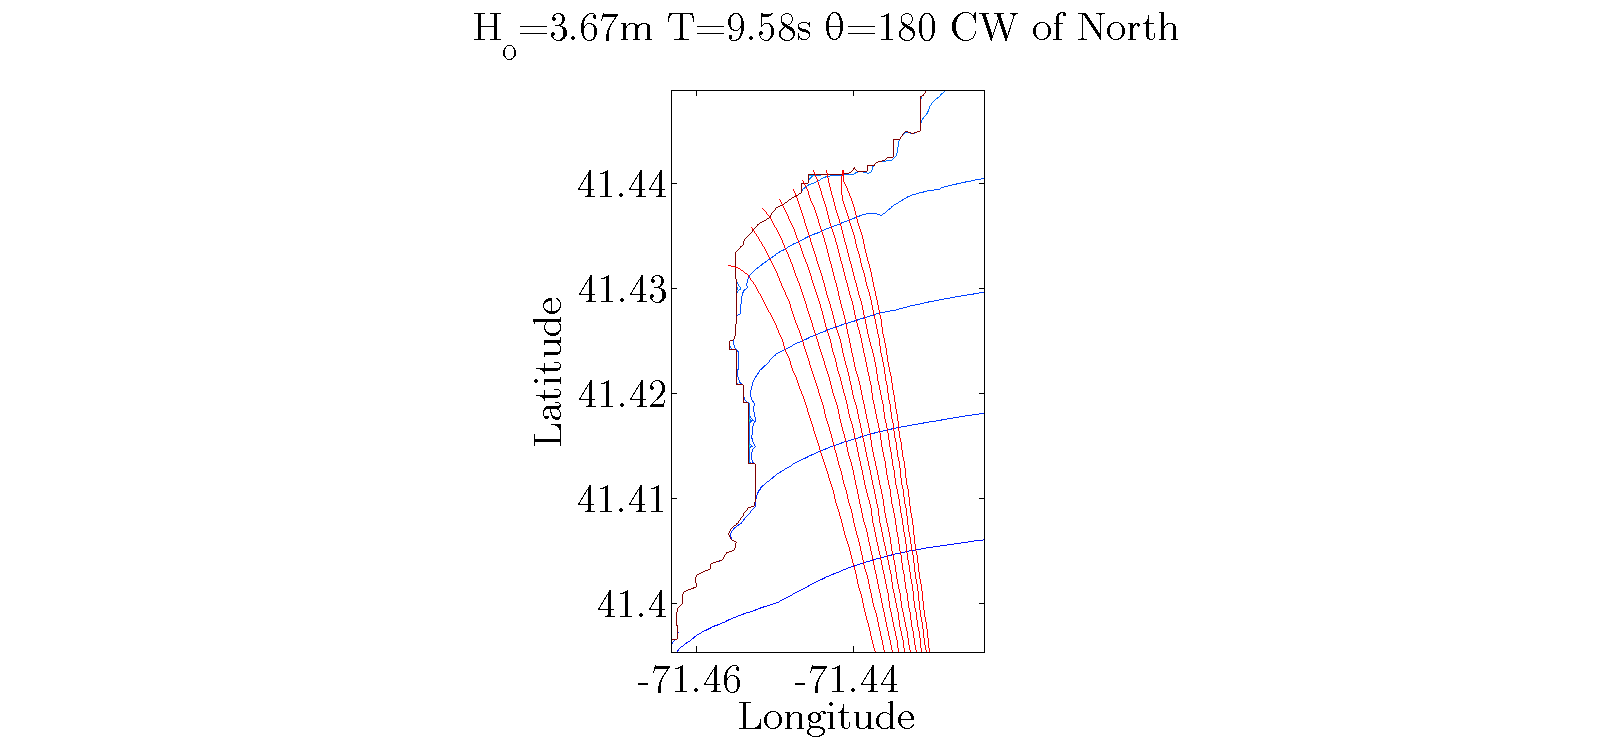
\includegraphics[width=0.6\textwidth]{./img/20y_180deg.eps}
\caption{Wave Ray 20y Expected Wave Parameters at 180 deg}
\label{fig:20y180deg}
\end{figure}

\begin{figure}[H]
\centering
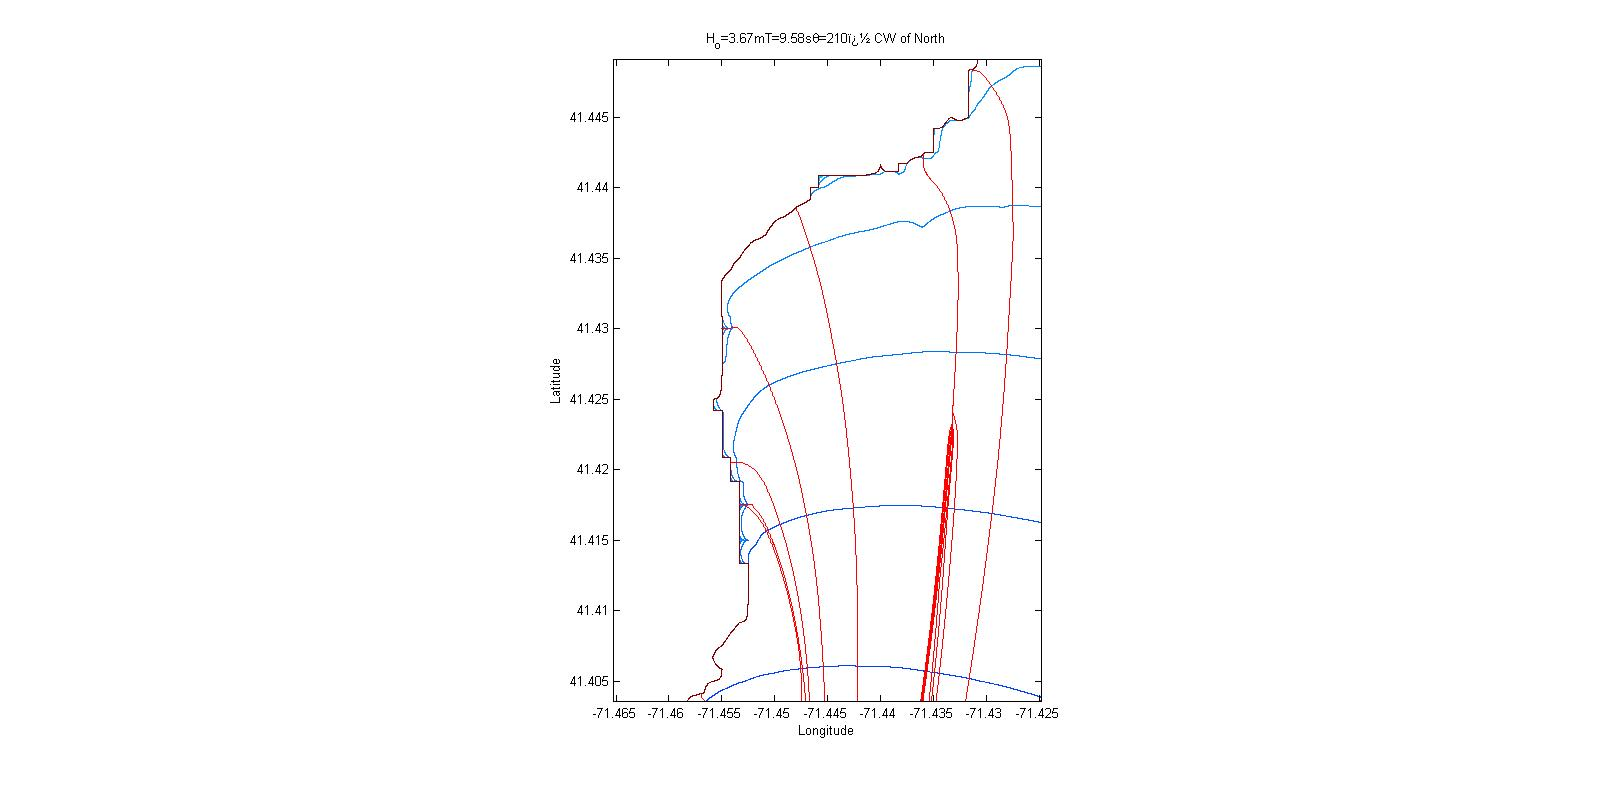
\includegraphics[width=1.0\textwidth]{./img/20y_210deg.eps}
\caption{Wave Ray 20y Expected Wave Parameters at 210 deg}
\label{fig20y210deg}
\end{figure}

Seen below, the simulated wave rays for the 50 year extreme waves were very similar to their 20 year counterparts. Narragansett Beach de-focused the few rays that hit the beach, and the degree of de-focusing can be observed to increase as the angle of incidence approached 210$^{\circ}$.

\begin{figure}[H]
\centering
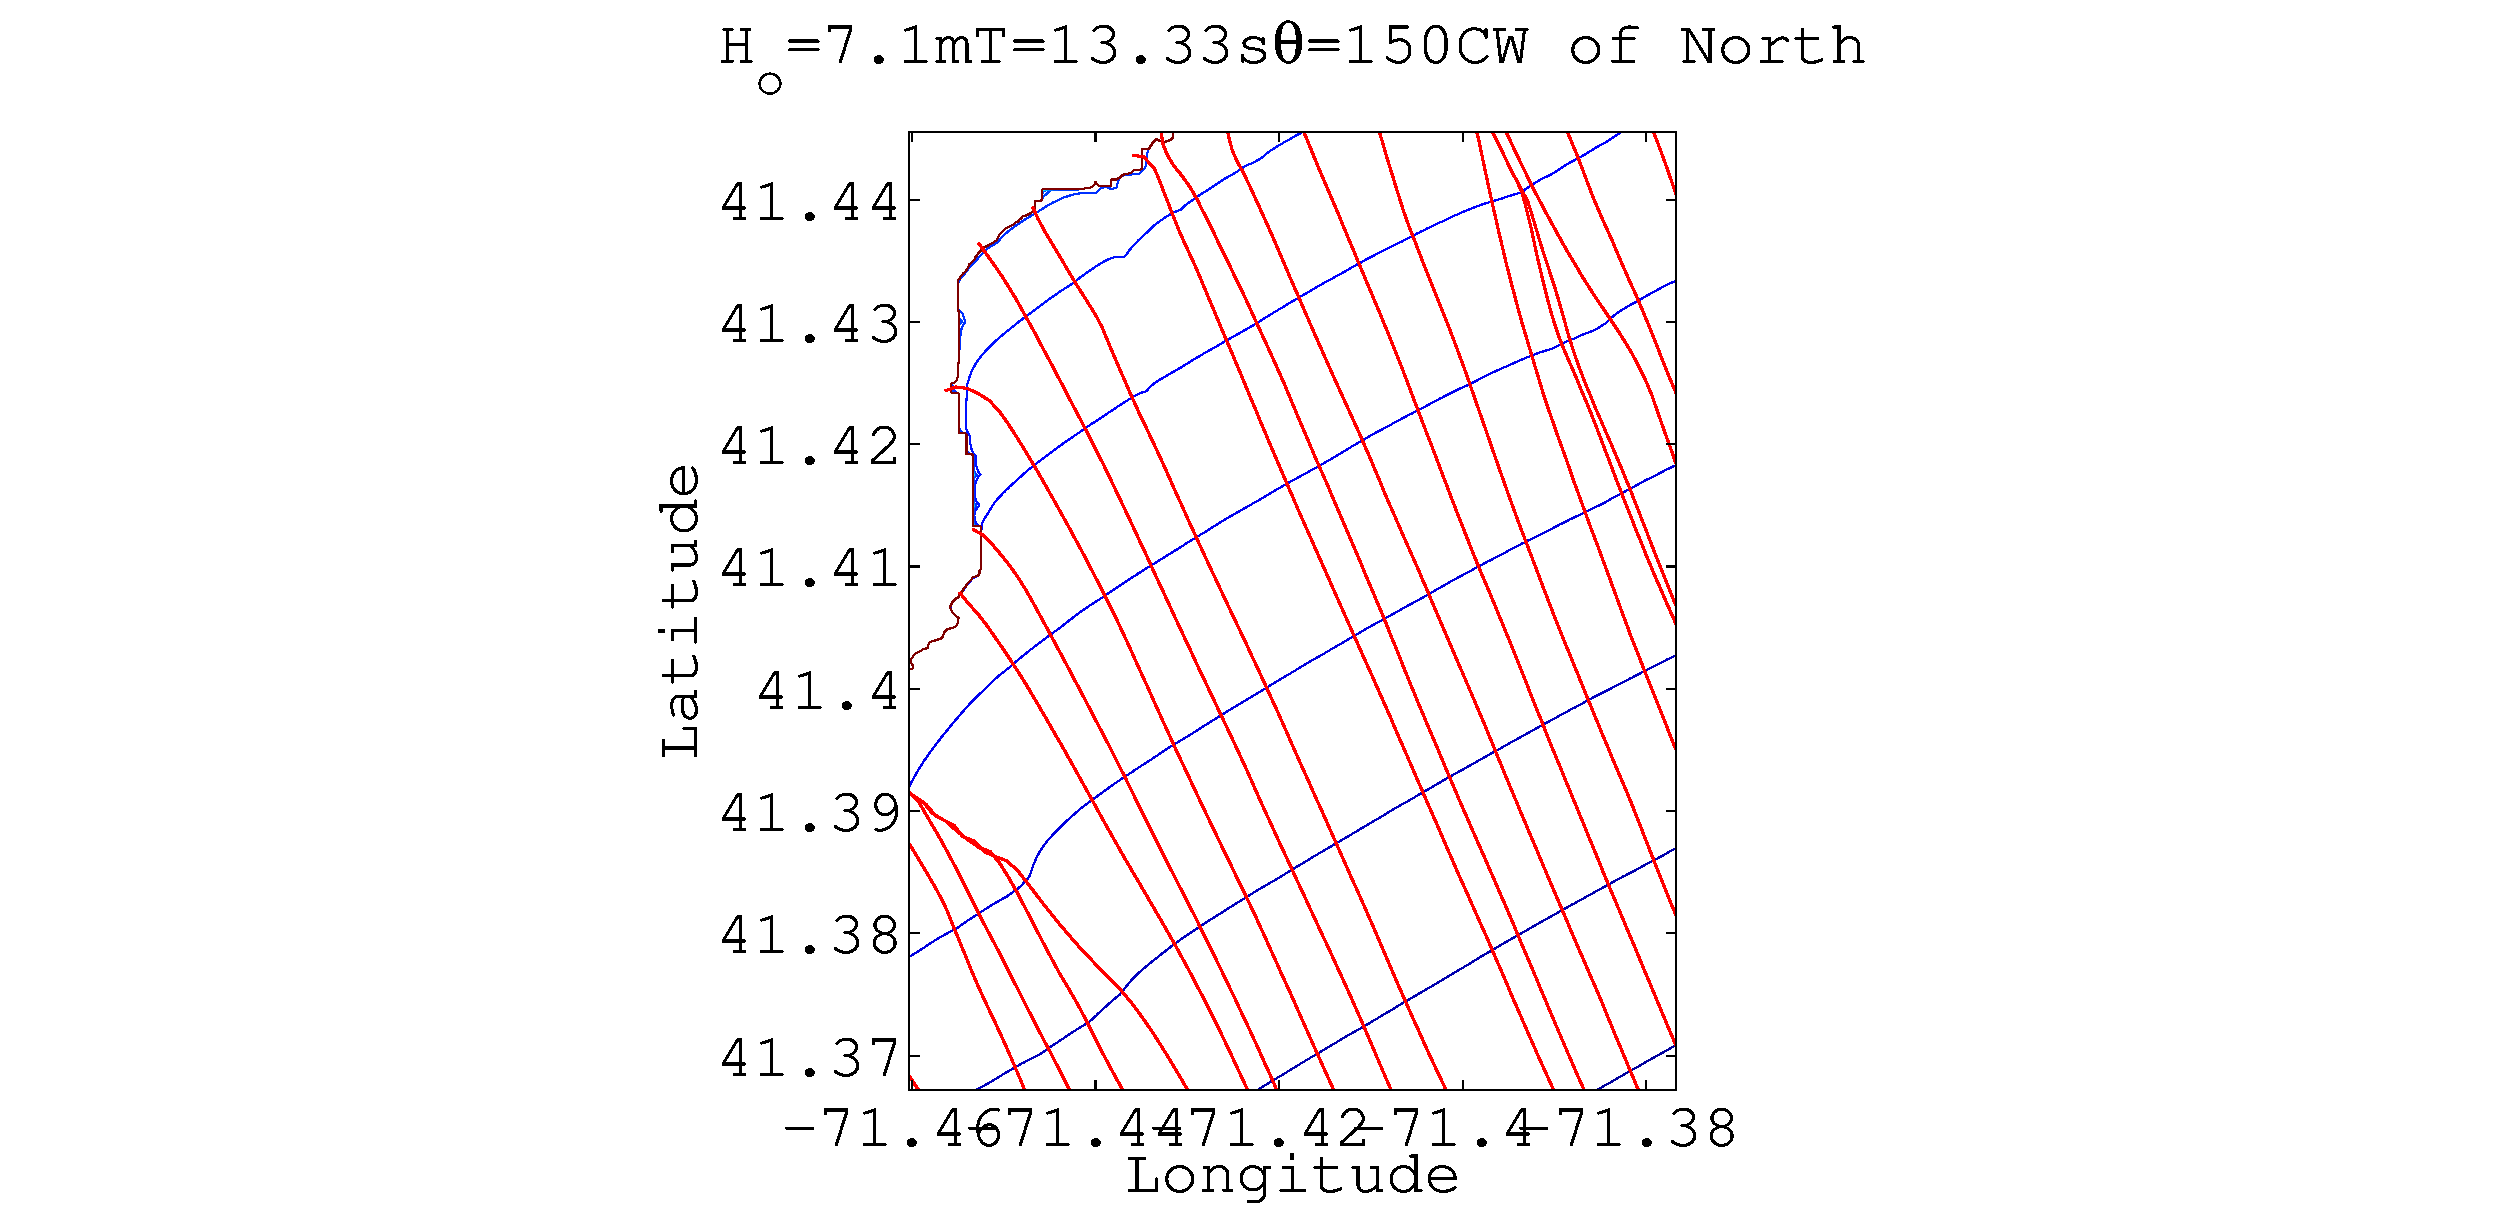
\includegraphics[width=1.0\textwidth]{./img/50y_150deg.eps}
\caption{Wave Ray 50y Expected Wave Parameters at 150 deg}
\label{fig:50y150deg}
\end{figure}

\begin{figure}[H]
\centering
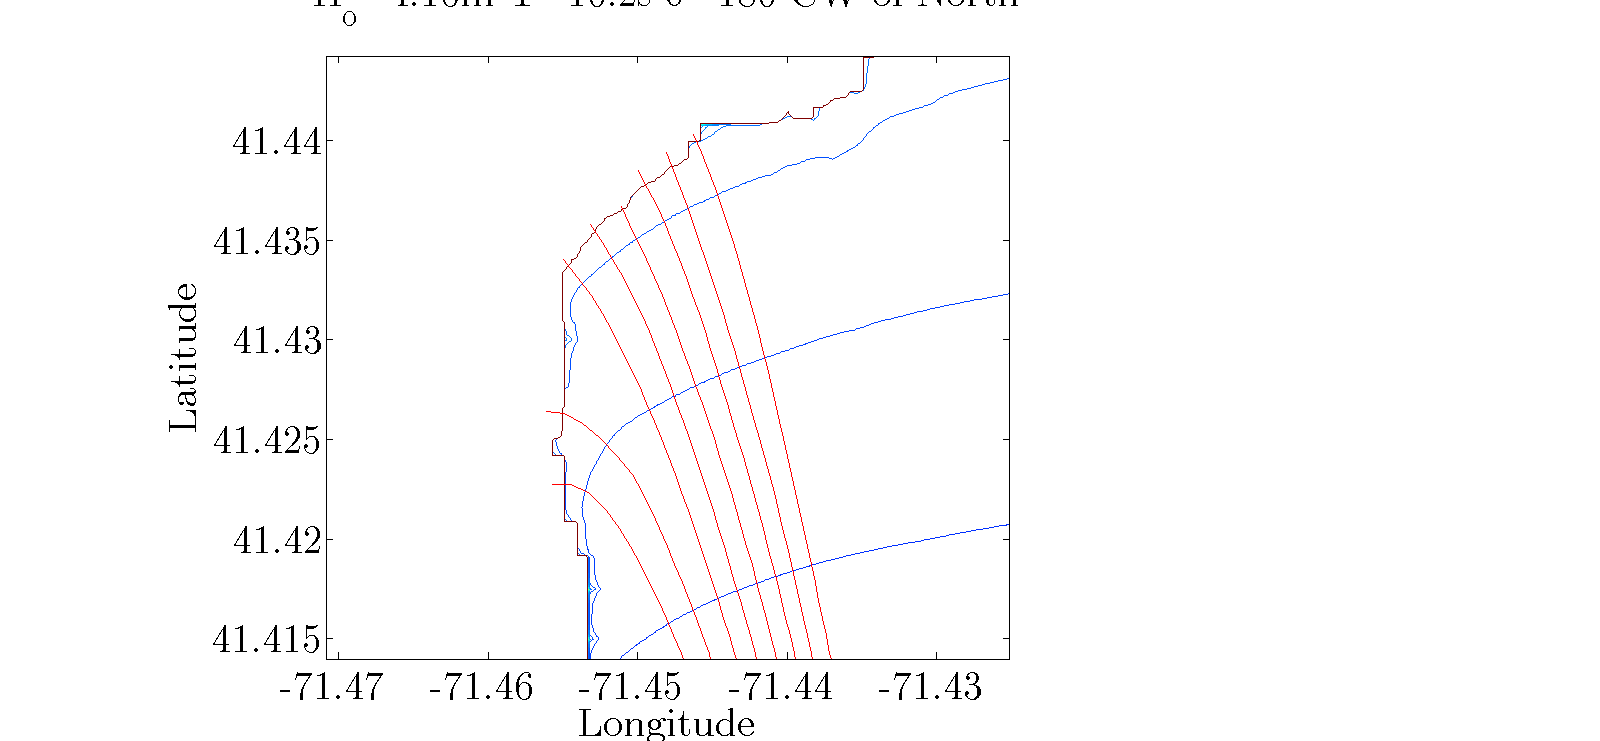
\includegraphics[width=0.6\textwidth]{./img/50y_180deg.eps}
\caption{Wave Ray 50y Expected Wave Parameters at 180 deg}
\label{fig:50y180deg}
\end{figure}

\begin{figure}[H]
\centering
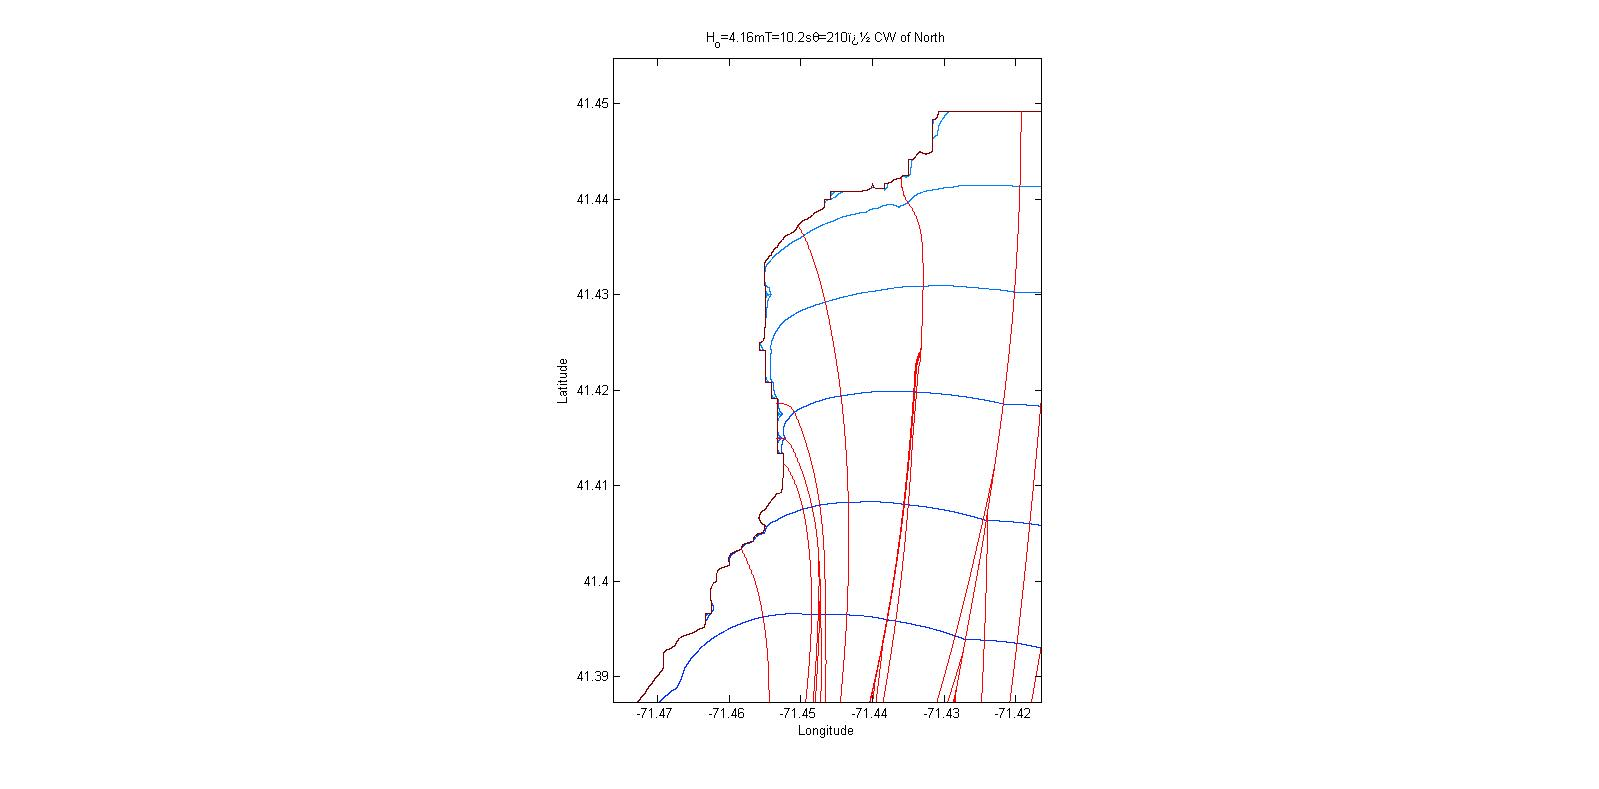
\includegraphics[width=1.0\textwidth]{./img/50y_210deg.eps}
\caption{Wave Ray 50y Expected Wave Parameters at 210 deg}
\label{fig:50y210deg}
\end{figure}

%Talkin bout sediment transport
Sediment transport 

%Talkin bout wave energy facility and location importance and such

%Talkin bout inclusion of diffraction model
Diffraction modeling would have influenced our 210$^{\circ}$ angle of incidence waves. Bloc

\section{Conclusion}